\documentclass[12pt,final,oneside]{fithesis}
\usepackage[slovak,english]{babel}
\usepackage[T1]{fontenc}
\usepackage{makeidx}
\usepackage{graphicx}
\usepackage{lmodern}
\usepackage{url}
\usepackage{caption}
\usepackage{listings}
\usepackage{color}
\usepackage{xcolor}
\usepackage[pdftex,bookmarks=true]{hyperref}
\usepackage{paralist}
\usepackage{textcomp}

\clubpenalty=300
\widowpenalty=300

\hyphenation{da-ta-base hy-po-nym me-ro-nym me-ta-da-ta HTMLCleaner}

% syntax highlighting

\newcommand{\bb}[1]{\textbf{#1}}
\newcommand{\code}[1]{\emph{#1}}
\newcommand{\n}{\lstinline|\n|}

\definecolor{javared}{rgb}{0.6,0,0} % for strings
\definecolor{javagreen}{rgb}{0.25,0.5,0.35} % comments
\definecolor{javapurple}{rgb}{0.5,0,0.35} % keywords
\definecolor{javadocblue}{rgb}{0.25,0.35,0.75} % javadoc
\definecolor{bashnormal}{rgb}{0.0,0.0,0.0} % bash

\lstdefinestyle{command} {
	language=bash,
	basicstyle=\ttfamily\small,
	keywordstyle=\color{bashnormal}\bfseries,
	stringstyle=\color{javared},
	commentstyle=\color{javagreen},
	numbers=none,
	numberstyle=\tiny\color{black},
	stepnumber=1,
	numbersep=5pt,
	tabsize=2,
	showspaces=false,
	showstringspaces=false,
	breaklines=true,
	captionpos=b
}

\lstset{style=command}

\lstdefinestyle{text} {
	language=bash,
	basicstyle=\ttfamily\small,
	keywordstyle=\color{bashnormal}\bfseries,
	stringstyle=\color{javared},
	commentstyle=\color{javagreen},
	numbers=none,
	numberstyle=\tiny\color{black},
	stepnumber=1,
	numbersep=5pt,
	tabsize=2,
	showspaces=false,
	showstringspaces=false,
	breaklines=true,
	captionpos=b
}

\lstset{style=text}

\lstset{
	language=XML,
	basicstyle=\ttfamily\small,
	keywordstyle=\color{blue},
	stringstyle=\color{black},
	commentstyle=\color{javagreen},
	morecomment=[s][\color{javadocblue}]{<!--}{-->},
	morekeywords={project},
	identifierstyle=\color{black},
	numbers=left,
	numberstyle=\tiny\color{black},
	stepnumber=1,
	numbersep=5pt,
	tabsize=2,
	showspaces=false,
	showstringspaces=false,
	breaklines=true,
	captionpos=b
}

\lstset{
	language=Java,
	basicstyle=\ttfamily\small,
	keywordstyle=\color{javapurple}\bfseries,
	stringstyle=\color{javared},
	commentstyle=\color{javagreen},
	morecomment=[s][\color{javadocblue}]{/**}{*/},
	numbers=left,
	numberstyle=\tiny\color{black},
	stepnumber=1,
	numbersep=5pt,
	tabsize=2,
	showspaces=false,
	showstringspaces=false
	breaklines=true
	captionpos=b
}

\makeindex

\thesistitle{Arquillian testing platform support for Android web and native applications}
\thesissubtitle{Diploma thesis}
\thesisstudent{\foreignlanguage{slovak}{Bc. \v{S}tefan Miklo\v{s}ovi\v{c}}}
\thesiswoman{false}
\thesisfaculty{fi}
\thesisyear{spring 2013}
\thesisadvisor{RNDr. Adam Rambousek}
\thesislang{en}

\begin{document}

\FrontMatter
\ThesisTitlePage

\begin{ThesisDeclaration}
\DeclarationText
\AdvisorName
\end{ThesisDeclaration}

\begin{ThesisThanks}
I would like to thank Karel Piwko, my leader in Red Hat Inc., for his valuable advices and insights during writing this thesis which helped me to understand the internal working of Arquillian framework a lot better. My thanks are going to Aslak Knutsen from Red Hat Inc. for the similar reasons.
\end{ThesisThanks}

\begin{ThesisAbstract}
The aim of this thesis is to design and implement an Arquillian container for Android devices, which is used during functional tests of web applications running at enterprise application servers. Investigation of integration testing of native Android applications via implemented Arquillian Android container is presented	.

This thesis is offered within the project ''Platform for cooperation in research and education with FI
MU in data processing'', registration number CZ.1.07/2.4.00/12.0049, in conjunction with activities of
the Association of Industrial Partners.
\end{ThesisAbstract}

\begin{ThesisKeyWords}
Arquillian, container, Android, ShrinkWrap, testing, functional, integration, extension, JBoss, enterprise, Drone, JavaEE
\end{ThesisKeyWords}

\clearpage
\thispagestyle{plain}
\par\vspace*{.35\textheight}{\textit{Identical units tested under identical conditions will not be identical on the final test after being buried under other components and wiring.} {\par}\hfill{Murphy's law}}

\MainMatter
\tableofcontents

\chapter{Introduction}
The result of one's activity in the manner of a tool or an application, which is to be used by him or by others, in order to be helpful and to fulfill the specified aim and before its introduction to production, has to be tested.

In context of the Murphy's law at the beginning of this thesis, we could ironically say that it holds in software engineering very strongly. Software engineering and development of software as such strives for quality in sense of absence of bugs and smooth integration into existing solutions or functionality of the product.

Quality engineering and testing methodologies in Java enterprise environment have been the subject of very vivid discussions. Couple of techniques as unit testing by testing frameworks as JUnit, TestNG and others have emerged and whole concept of programming like test driven development or eXtreme Programming have been propagating widely. 

Besides the unit testing as the very basic principle of testing, integration and functional testing is as important as the former one. In the zoo of frameworks and plethora of tools for JavaEE platform, it is important to be sure not only components of the software solution work as expected but also their interconnection, communication and integration with application containers and other enterprise layers is functioning as well.

While trying to doing so, we realize very early that it is not easy task and in lot of cases not even possible. The reason is that we are are trying to bring the whole runtime into our test so we are orchestrating all layers trying to fake the original target environment in which our product will be running. The orchestrating and faking all complex enterprise services as dependency injection, messaging or database performance and simulating system errors and communication between multiple entities in our software solution is heroic work and it is not possible to simulate exactly the same scenario multiple times and repeatedly.

This thesis aims to improve functional and integration testing of web and native Android applications on JBoss platform cooperating with Android platform. The crucial role in the functional and integration testing plays Arquillian testing platform.

Arquillian testing platform provides a way by which we can get rid of aforementioned impossibilities of testing cases. The core principle which stands behind Arquillian is the philosophy of bringing the tests into target runtime and not otherwise - the typical way of dealing with tests so far. This simple switching of point of view makes whole enterprise testing in JavaEE revolutionary. 

It is important to realize the essential component without which testing by Arquillian would be meaningless - application container or application server. The application container is a place where, roughly speaking, application is deployed and made accessible for users. Arquillian is container agnostic, which means it does not matter against what target environment the application is tested.

Arquillian is not only a tool for rigid testing of enterprise services and technologies but it also provides a way how to make testing via automating web browser in case we are trying to test web application. There are already solutions how to automate web browser such as Selenium - the pioneer of automated testing frameworks. JBoss community developed a tool which is based on Selenium of name Arquillian Graphene. Arquillian Graphene is designed as set of extensions for Selenium WebDriver.

The functional testing by automating web browsers has its counterparts in Android platform, to name a few, Solo or Robotium. This thesis tries to focus on integrating these tools into Arquillian environment and to make testing of Android application as similar as possible so we can gain from advantages of Arquillian in this direction too. 

\chapter{On software development processes}

In this chapter, we are discussing two most widely-known approaches to the development of the software - serial (or sequential) development model and iterative development model. Both models will be described and their pro et contra will be discussed. We will discuss both models in sense of their attitude to testing process or methodology too.

	\section{Serial development process}
Serial development model is a traditional software development process. This process is commonly used in the most development projects. The main description of the process is that it is divided into set of activities. When one set is finished, the other starts. When all sets of activities are done, the whole development process is considered to be about its end. The development model of such pattern is also called waterfall process since there is no easy way how to go back in the development and return to some previous stage. There is basically no way how to switch to the older stage or at least it is used to be challenging and more resource, time and finance demanding.

The process has typically five phases as it is shown in the next figure. To name them, they are called: requirement analysis, design, implementation, testing, installation and maintenance.\\

\begin{figure}
	\centering
	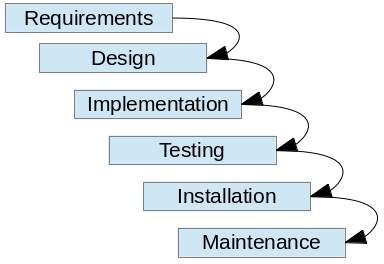
\includegraphics[width=70mm]{img/waterfall.png}
	\caption{Waterfall development process}
	\label{fig:waterfall_process}
\end{figure}

\begin{itemize}
	\item[\textbf{Requirements analysis:}] This step is the most important phase of the waterfall model. In this phase, all customer requirements are gathered, involving clear definition of the customer goals and expectations. Requirements analysis is also the place where the understanding of the customer's context and constrains are specified. To obtain all these information, customer is involved into this phase very actively since he represents the only source of information which developers have access to. The outcomes of the analysis are persisted into so called software requirement specification (SRS) of the application. The SRS is describing the behavior of the system entirely and in the great depth and detail. The SRS in used in the next phases actively. 
	\item[\textbf{Design:}] After SRS is available, software architects and designers are about to start the designing the overall look of the software solution. The design phase involves defining the hardware and software architecture, specifying performance and security parameters, designing data storage containers and constraints, choosing the IDE and programming language, and indicating strategies to deal with issues such as exception handling, resource management and interface connectivity. The output of this stage is called SDD - software design description.
	\item[\textbf{Implementation:}] After the final product is fully designed and all requirements of the customer were incorporated, the implementation of the product takes its place. The input to the implementation phase is the SDD of the system from the design phase. The implementation phase is the logical continuation of the design phase where the product is built.
	\item[\textbf{Testing:}] Testing phase, which follows the implementation phase, verifies that the application or the software solution is meeting requirements put on the product in the first phase and additionally that the application is bug free. The test cases are written in order to evaluate the implementation. There are various categories of testing - unit testing, system testing or acceptance testing. If some errors, bug or malfunction is observed, it is up to the development team to refactor the code, incorporate changes and do tests once again until the product is valid and ready to be installed.
	\item[\textbf{Installation:}] Installation phase actually delivers the developed and tested product to the customer. It can be installed by customer itself, development team or by other third party.
	\item[\textbf{Maintenance:}] Waterfall model is finished by maintenance phase which follows installation phase at the client site. There is not any functionality added. This phase is used to tweak the product in a such way that its performance is improved and attributes of the product are modified to better reflect clients execution environment. 
\end{itemize}
To sum the sequential (serial) development models, the main idea behind this kind of models is to design and project every single aspect of the final product in very deep details. Only after very careful specification of what is going to be done, further steps are taken, ignoring the client or customer from the development process, when all possible information are extracted. The reason of doing so is to reduce wasted time by avoiding the need to go back and make corrections which are used to be costly.

The main disadvantage of this approach is that the never-go-back mentality of a serial process makes it very hard to maintain and build adaptable and modifiable code in the future. The sequential model tries to avoid changes while the product is being developed.

On the other hand, these types of development processes are suitable for projects where it is known keeping the room for changes in the future is not necessary or not required. In addition, having a precise idea of what application will consist of and what requirements are put on it can uncover notable flaws that might occur in later stages.

	\section{Iterative development process}

Iterative development processes can be viewed as direct opposite of sequential ones. Functionality is added by iterations, from very basic to more advanced, from simple to more complex. In this section, we will discuss two approaches which are very popular among iterative development processes. Tests coders are preparing while they are developing the actual application is the activity which is these days not considered to be only the side effect and the evil which has to be eventually done, but it is a way and strategy how to develop as such. This approach to the developing is called test driven development (TDD). Test driven development plays very nicely with another very popular term which symbolizes whole principle of coding - eXtreme Programming (XP).

	\subsection{Test driven development}
Test driven development is a way of programming when you are writing your tests firstly and before any single line of code of the target application is written. The first step is to add quickly a test which has to fail upon first run. Only when a test is written, you write the application code and run that test against what is written so far to get rid of failing test and have the test which passes. If we run the code and that code is still failing, we have to return back to coding, repair the code and run tests once again. Only when tests are passing, we can write other tests which test different functionality and do the same process again.

The process just described is called TFD (test-first development). Test driven development is understood as a TFD with refactoring. This approach to coding process is completely different from what majority of programmers are used to. The traditional view is to code some subset of the functionality and then to write tests to see if it fails or passes and react accordingly. The importance of getting tests written in advance is in the way how we think about the design of the application. We are trying to make our design the best possible in advance thinking about how some particular design is going to be helpful for us. TDD calls for the opposite way. We are focusing on new functions so every other functionality added constantly improves our design and just fits our needs.

\newpage
There are two levels of TDD:

\begin{itemize}
	\item{\textbf{Acceptance TDD (ATDD):}} With this approach, we are writing single acceptance test and just enough production code to satisfy that test. The goal of ATDD is to specify detailed, executable requirements for our solution on a just in time (JIT) basis. ATDD is also called Behavior Driven Development (BDD).
	\item{\textbf{Developer TDD:}} With developer TDD we write a single developer test, sometimes inaccurately referred to as a unit test, and then just enough production code to fulfill that test. The goal of developer TDD is to specify a detailed, executable design for our solution on a JIT basis.  Developer TDD is often simply called TDD.
\end{itemize}

The result of programming TDD way can be summarized in these points:

\begin{itemize}
	\item{Our development environment must provide rapid response to small changes.}
	\item{Unit tests has to run fast (they have short setups, run times, and break downs).}
	\item{Unit tests run in isolation, we should be able to reorder them and no test is dependent on the other.}
	\item{Tests are using real data and are executed in simulated production environment.}
\end{itemize}	

	\subsection{Extreme Programming}
Extreme programming is one of the several popular agile processes. The extreme programming style of the software development is hard to describe in it's entirety but in order to complete the image of how the programming can be and is done these days, we have to evaluate it.

What is one doing if he develops in the extreme way? To describe his attitude superficially, the first of all, so-called extreme developer starts to code as soon as possible and does not think about the overall design of the application in advance. At the first look, this basic strategy can appear to be dangerous or wrong at all from the academic point of view where sequential development strategies or waterfall-like strategies are used rather often, but this approach has some undeniable advantages and desirable consequences which are highly valuable and will be discussed.

When developer team starts to work on some project, the very typi\-cal beginning is to plan everything into details and the significant amount of time is spent with the customer describing and specifying what output he wants to eventually see. The big problem of this app\-roach is the uncertainty of the output. With the best intentions to catch users needs and requirements, nobody is able to be completely precise about how the final product will look like. It is not the fault of the development team, meaning its disability to understand what the customer wants. Typically, a customer or a consumer of an application even does not know what should be done. The customer is used to have only vague idea what kind of problem the application should solve and he is willing to change the goal, design and requirements as the application is under the construction.

For these reasons, the typical scenario mentioned in the sequential models, which is to consult everything in advance, is flawed and not sufficient. It is often the case that after the customer declares what he wants and the consulting is done, the second time we face the customer is upon final delivery of the product. In the extreme programming paradigm, the customer is the essential part of the developing process and he is participating all the time application is under construction. Of course, one has to design and plan at least something, there has to be clear borders e.g. the problem domain the application will be dealing with, but every further details of how it should be done later are meaningless.

The extreme way of programming is also about doing plans but the strongest attitude can be sum up in the slogan "Do the Simplest Thing that Could Possibly Work" and the abbreviation YAGNI which stands for "You Are not Going to Need It".

While the meaning of the first phrase is clear, the mentioned abbreviation has to be clarified. When we are developing the application, we are very often ending up with the design which is over-engineered and after completion of some problem, we have coded infrastructure for solving problems which do not even exist yet and we provided functionality which is not necessary. We likely think that by coding a lot in advance, we will be free from implementing it once there will be the need to do so. We are keeping doors widely open to hook and modify almost everything or at least with the smallest pain. But the question is - what if that situation never happen? By implementing the functionality we do not need, we will face two very probable outcomes. The~first is the need of taking care of the unused code and pulling it all the way with us while we develop which adds additional complexity to the  existing code and by this way it becomes more error prone. The second is the fact that our imagination of what user wants is completely out of range so we are wasting the time.

The key concepts of the extreme programming can be summed up in the following points:
\begin{itemize}
	\item make frequent and small releases
	\item a project is divided into iterations
	\item no functionality is added early
	\item refactor whenever possible
	\item code the unit test first
	\item integrate often
	\item all code must have unit tests
	\item when a bug is found, tests are created
\end{itemize}   

Extreme programming suffers from some drawbacks too. Extreme programming is more code-centered then design-centered so it is more suitable for smaller projects or in projects which do not span over more development teams. Using extreme programming in such scenario would be more counterproductive then useful. Since extreme programming lacks design documentation in the great detail because it varies constantly, we are short of reuse opportunities. Extreme programming does not maintain quality plan. Having of such plan reduces time reserved for testing. Extreme programming spends huge amount of time on testing process. 

In spite of mentioned drawbacks, extreme programming can be successful because it focuses on the customer's satisfaction in every moment. We could know that some feature will be needed in the future, but we are not going to implement it right now, even it is very easy to introduce and implement, because it is not necessary in the present moment. When the time comes, the code can be refactored and missing functions added and it does not matter if we are in the late period of the life cycle of the product. The architecture and design of the project or its part is kept as simple as possible so further modifications and additions can be done over the skeletal design - enabling continuous refactoring.

	\section{Necessity of continuous integration}
	
Both models of software developing we discussed earlier - sequential development process which of representative is the waterfall model and iterative development models as TDD and XP - have to integrate the functionality and code into the already existing code base.

While in the sequential development process the integration phase is standalone, long term and time consuming event, it is often only the bad practice and habit why it is so. The key to the successful and painless development scenario is to integrate part by part, code by code and day by day as iterative approach suggests. This approach is rarely taken in the case of sequential development. On the other hand, TDD and XP approach is very suitable for so called continuous integration. We will describe what continuous integration (CI) is and how can be helpful in both development models mentioned in the previous sections.

We can explain continuous integration process on the example in context of XP as well as waterfall on the next figure:

\begin{figure}
	\centering
	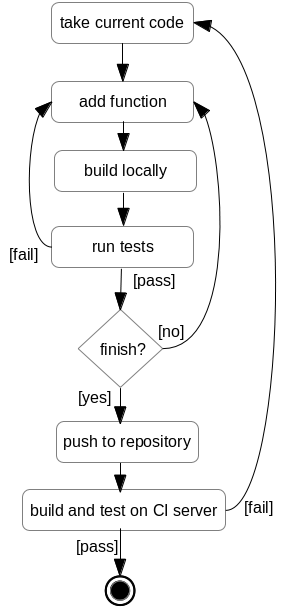
\includegraphics[width=70mm]{img/ci.png}
	\caption{Continuous integration}
	\label{fig:ci_process}
\end{figure}

\newpage

The very first goal in order to do CI is to have a central place where the all source code and resources necessary to build and run the project are stored. It is important to realize that a source code repository should contain everything in order to build the project successfully and not only source code itself but whole tools, scripts and resources. In the ideal state, we should check out the code from the repository on the clean (developer) machine and run tests, build application and run it from scratch. The most popular distributed source code repository nowadays is Git, so a reader can bear in mind this kind of repository while reading further.

When a developer clones a repository or when he updates his local repository to the newest commit to synchronize his local repository with the main repository, he starts to add a functionality into the code. It does not matter what kind of functionality or change it is really, but let's say, for the sake of the argument, he is trying to add some business functionality or fulfill some user's story card.

While doing so, he writes the tests, as the TDD approach is advising, builds the project locally, ensures himself that tests which verify new functionality are failing and starts to implement what is necessary.

He builds the whole project or module of the application as he develops, checking his progress. He repeats this process while tests are failing. When they stop to do so, it is a sign that the functionality is done and he can commit and push to the remote repository where everybody checks the source code from.

By committing to the remote repository, his work is done only partially. It is so because there is a continuous integration server which fetches the whole repository, build the project and runs all tests again.

The necessity of continuous integration server is determined by distributed nature of the source code repository. More then one developer can check the source code so more then one developer can work on the project simultaneously which means that after both developers commit their work, after resolving possible clashes which originate from the work of both of them, we have to build and test once again since there can be still a possibility that some artifacts or resources are not pushed to the repository so build which is run externally from development machine can fail.

Activities related to the continuous integration can be handled automatically or manually. Automatic builds can be executed on some preferred interval or when changes in the main repository are detected.

After getting the initial image of the CI, when one wants to use CI, he needs to build and maintain an infrastructure which: \textbf{ref na fowllera}

\begin{itemize}
	\item{contains a single source repository}
	\item{automates builds}
	\item{makes builds self-testing}
	\item{builds the newest code on the integration machine}
	\item{keeps builds fast}
	\item{tests in production environment}
\end{itemize}

As mentioned earlier, source code can be tracked in Git but other source code repository can be used as SVN or Mercurial.

The automation of the builds can be provided by Java building tool called Maven. The role of the continuous server can be handled by the Java software component called Jenkins.

It is clear that the main stress will be put on the fact that the builds and tests have to be done fast because they are done frequently. If our builds, functional and integration tests took tens of minutes or hours, it would be useless to use the TDD and XP in the JavaEE development. Tests are driving the development. Testing \emph{is} development. We are doing incremental changes, we are adding functionality frequently and piece by piece and we also integrate on-the-fly so we know better every moment how is our project doing which is only hardly doable in the sequential development model when the integration exhibits at the end of the implementation and refactoring of the code is very hard. Continuous integration process encourages to do smaller steps and to check how we are doing, keeping the overview of the project up to date.

We are also trying to do all the tests in the target environment so we need take our tests to the runtime and not otherwise as it was discussed in the previous sections.

\chapter{Testing in JavaEE environment}

The next chapter will discuss existing tools and techniques which are used in connection with testing process and infrastructure in Java EE environment. We are dividing these tools which will help us to describe the context of Arquillian testing into three categories. These tools and software compilations are helpful for ongoing explanation of Arquillian testing platform and a reader will be prepared to understand whole model of Arquillian testing much better and smoother.

	\section{Tools used in JavaEE environment}
	
		\subsection{Maven}

Maven is so-called build automation tool. Maven is written in Java programming language and it is massively used in Java ecosystem. The main purpose of Maven is to describe the software project - its build, its development, testing and release life cycle and other projects on which our project is dependent with version management in mind.

By default, for every Maven-based project, the structure of directories is the same for all of them. 
In source-related directories, Java packages are saved. The default directory layout for a project is as follows:

\lstinputlisting[style=text,caption=A Maven project directory layout]{src/maven_layout.txt}

A typical Maven build life cycle consists of sequence of phases - \texttt{prepare-resources},\texttt{compile},\texttt{package},\texttt{install}. There are always \texttt{pre} and \texttt{post} phases which can be used to register \texttt{goals} which must run prior or after a particular phase.

Maven has following three predefined life cycles - \texttt{clean}, \texttt{default} and \texttt{site}. \texttt{clean} life cycle cleans a project, \texttt{default} life cycle builds a project and \texttt{site} life cycle builds into \texttt{target} directory complete web site representation of a project as it generates e.g. Java documentation (javadocs).

A \texttt{goal} represents a specific load of work a plugin has to execute and doing so contributes to the building and managing of a project. The order of goals is defined by default settings which could be overridden~- we can easily define our own actions which are being to be executed upon project build. The order of execution depends on the order we specify phases and goals on the command line.

Maven is mostly ridden by command line command \texttt{mvn} after which phases and goals follow. Phases and 
goals can be chained. A goal of some plugin can be executed as:

\lstinputlisting[style=command]{src/maven_execution.sh}

For example, when we want to clean project, to delete the build, we have to trigger \texttt{clean} phase. This 
phase deletes \texttt{target} directory, by default. If we want to build sources and make a \texttt{jar} package, we need to invoke \texttt{package} phase. Since goals can be chained, we execute:

\lstinputlisting[style=command]{src/maven_clean_package.sh}

When specifying \texttt{package} phase, all goals and phases which proceed this phase are executed as well. For example, \texttt{test} phase is executed after \texttt{compile} phase but before \texttt{package} phase, so we are sure tests are executed and software does what it is supposed to do before package is created.

The second very important role of Maven is to track \textit{dependencies}. Dependencies are stored in \textit{repositories}. By default, dependencies are downloaded from main Maven repository\footnote{http://search.maven.org/}. After downloading dependencies we need to satisfy our project with, they are stored in a cache repository at a development computer so that way there is no need to download them over and over again. A dependency is an \textit{artifact} which has exact and unique \textit{coordinates} over all dependencies. Every artifact has coordinates of the form:
\begin{center}
	\begin{minipage}{.7\textwidth}
		\lstinputlisting[style=command]{src/dependency_coordinates}
	\end{minipage}
\end{center}
Every artifact belongs to some group. This is reflected via \texttt{groupId} element. An artifact can have different versions. We can not import two same dependencies each with different version. \texttt{packaging} element specifies how project is packaged. The most common values are \texttt{jar} or \texttt{pom}.

All project definition is stored in file \texttt{pom.xml} which is a shortcut for \textit{project object management}. Maven finds \texttt{pom.xml} automatically when invoked in the same directory as \texttt{pom.xml} is saved. The very basic \texttt{pom.xml} file for the illustration purposes to reflect written previously is following:

\lstinputlisting[language=XML,label=pop-pipe,caption=A simple pom.xml file]{src/pom_example.xml}

Dependency can have a parent, in that case, project's \texttt{pom.xml} it is not a \textit{top-level} \texttt{pom.xml}. A parent normally serves as an aggregator of different artifacts which are logically grouped but each artifact has its own responsibility and specific meaning in a project. After parent definition, coordinates of an artifact follows and finally we see this artifact depends on \texttt{junit} artifact of particular version and \texttt{scope}. When \texttt{scope} is not defined, it means that dependency is on classpath during compilation time, when \texttt{scope} is set to \texttt{test}, it means this dependency will be on classpath only during testing phase of the project - when we execute Maven as \texttt{mvn test}.

In Maven universe, beside ordinary POM files, there are also so-called \textit{BOM} files. BOM stands for \textit{bill of materials}. It is a POM file where only dependencies are specified so we can easily include BOM dependency into \texttt{pom.xml} and all dependencies which are specified in BOM will be imported to \texttt{pom.xml} as well. We can gather well known group of dependencies and import only one dependency which covers them all in order to provide more brevity and management convenience.

Maven is very helpful tool which in Java EE environment enormously simplifies project management, dependency tracking and artifact retrieving and hides complexity of a project dependencies. The managing of a project life cycle would be very time demanding and error prone task since we would have to specify everything manually. 

		\subsection{ShrinkWrap}

ShrinWrap is very simple but powerful tool. ShrinkWrap is Java library which provides a mechanism for constructing  archives as \texttt{jar}, \texttt{war} or \texttt{ear} programmatically and very easily. This is possible because of fluent API on which ShrinkWrap relies heavily and it is de facto the only way how to use the library. ShrinkWrap is standalone library and it does not depends on any external library. It needs just JRE5+ runtime.

The advantage of using ShrinkWrap is the easiness of creating custom archives. Archive file is built in a memory and written to any target via so called \texttt{exporter} afterwards. Resources which are added to final archive are located on class path.

ShrinkWrap is very sought-after tool since we can exactly specify, class by class and resource by resource, how the deployment to application server will look like and drive very subtle class path isolation. This fact is not true every time. When we are creating the archive, it is common resources and classes which are not needed are bundled into final package as well. This fact can negatively influence functionality and run time of a deployed package e.g. by not finding desired resources or because of some clash. While testing the software, we need to isolate test cases and find the smallest common denominator which satisfies all dependencies and get rid of unused resources. This approach also encourages TDD and unit testing - we are only testing classes we are interested in and we are not taking any garbage which could influence result of the test unpredictably with us. The example of constructing \texttt{jar} file programatically via ShrinkWrap fluent API is following: 

\lstinputlisting[language=Java,label=pop-pipe,caption=ShrinkWrap fluent API]{src/shrinkwrap_archive.java}

The newly created \texttt{jar} file is stored in a generic \texttt{Archive} at line 5. The entry point to dealing with the library is \texttt{ShrinkWrap} class. We specify we want to create \texttt{JavaArchive}. This class has to extend generic \texttt{Archive} class (line 3). After these information, we are simply adding classes, packages or resources as manifest files into the archive, which will be persisted in \texttt{test.jar}.

Creating deployable archives with ShrinkWrap is very convenient way how to precisely specify and construct an archive which just meets our needs. We are able to put everything we want into the archive under the construction so we can bundle there our own resources at will as well as we can isolate or delete any resources and classes we want in order to strip an archive to bare deployable minimum.

		\subsection{Jenkins}

Jenkins in a continuous integration (CI) tool written in Java language. Jenkins is an open source project. The purpose of Jenkins is to provide continuous integration services for development of a software. In it's core, it is server-based system running in some kind of servlet container as Apache Tomcat.

A testing machines we are testing software under development at are called \textit{slaves nodes}. A slave has various parameters such as amount of memory available, operating system, system architecture, installed versions of Java Virtual Machines and so on. We can then register various integration servers at will and we can specify on which slave nodes we want to test our software according of their capabilities and our requirements. More often we do not specify directly which slave node we want to use. We only tag slave nodes by its capabilities and specify a query via which appropriate nodes are selected automatically.

Tests can be run at more then one slave node since we may want to know if our software is capable of running under various circumstances, e.g. if it works without issues on multiple configurations so we mimic heterogeneous target environment.

After the filtering on which node tests are going to be executed, the actual source code of our interest has to be checked out (or cloned) from central source code repository as Git\footnote{http://git-scm.com/}, SVN\footnote{http://subversion.apache.org/} or Mercurial\footnote{http://mercurial.selenic.com/}.

Build of the tests can be triggered by various means, it can be triggered periodically on some predetermined frequency (e.g. every two hours) or it can be triggered automatically by every commit we push into source code repository. Jenkins uses concept of \textit{downstream} and \textit{upstream} builds so tests or builds of downstream project is triggered when all upstream projects are built and tested without issues. Local copy of source code is cloned at slave node and Jenkins executes tests and reports results back to Jenkins master server.

Jenkins plays significant role in Java EE environment and is very widely known to Java-oriented community. Jenkins plays very well in connection with Maven-based projects. Jenkins can test and build virtually any Java project. There is the effort to make various bindings to support .Net\footnote{http://www.microsoft.com/net} or Scala\footnote{http://www.scala-lang.org/} projects with various success.

Continuous integration system as Jenkins offers the very first prerequisite for successful and painless iterative development and reduces integration testing significantly.

		\subsection{JUnit}
		
After having an arbitrary Java project based on Maven and setting up infrastructure for continuous integration testing via Jenkins, where source code is cloned or checked out from distributed source code repository, we need to perform testing itself. The most popular testing tool for Java is JUnit. JUnit is an instance of the xUnit architecture for unit testing frameworks.\footnote{http://junit.org/}.

JUnit tests, as the name of the framework suggests, are meant to be unit tests. As previously stated, in TDD model, which is often used in XP, unit tests are written before the code itself is created so only when tests are passed, code is considered to be finished. The very central point of the unit testing is to show that each part of the program behaves correctly. Only after that, these parts are integrated together.

JUnit is added to Maven-based project as a dependency. All tests reside by default in \texttt{src/test/java} and resources needed for tests under run, if any, are located in \texttt{src/test/resources}. From Maven point of view, tests are executed as \texttt{mvn test}.

The example of simple JUnit test is following. Its core features and life cycle of the test class will be discussed further.

\newpage

\lstinputlisting[language=Java,label=pop-pipe,caption=Example of JUnit test]{src/ExampleTestCase.java}

A unit test is distinguished by JUnit when a test class is annotated with \texttt{@RunWith} annotation. Argument of \texttt{@RunWith} annotation is so-called \textit{test runner}. Test runner specifies how exactly test class, in our example \texttt{ExampleTestCase}, is treated. \texttt{org.junit.runners.JUnit4} is the default runner for JUnit. It extends \texttt{BlockJUnit4ClassRunner} in the same package. Every runner has to extends this base runner. Custom JUnit runners are changing the default behaviour of the test execution.

Every test case consists of particular unit tests. A test is a method annotated with \texttt{@Test}. All tests have to be \texttt{public void} methods without any arguments. The \texttt{@Test} annotation can have the argument \texttt{expected} which tells that this method is expected to result with thrown exception, for example in our case \texttt{IllegalArqumentException} at line 28. We are testing very basic functionality of \texttt{Adder} class which just adds arguments in \texttt{addPositiveNumbers} which input have to be two non-negative numbers, which is not the case. So this method is expected to throw the exception we are catching with \texttt{expected} argument. If, by any chance, our adding method passed, \texttt{fail()} method from JUnit would followed. This method ends test as failed.

Tests can be ignored with \texttt{@Ignore} annontation as shown at line 34. This test will be skipped upon test case execution.

We can define additional actions before and after test case class. These actions are executed once. They are called \textit{test fixtures}. Methods have to be annotated with \texttt{@BeforeClass} and \texttt{AfterClass} respectively. We can also specify what has to be done before and after every particular \texttt{@Test} method by \texttt{@Before} and \texttt{@After} annotation respectively. Class text fixtures have to be static methods.

It is important to realize that before every invocation of \texttt{@Test} method, JUnit instantiates whole new test class so \texttt{Before*} and \texttt{After*} methods are very handy when we do not want to repeat ourselves. We just put common set up into these methods and we are done, as shown in our simple \texttt{@Before} method.

The most common way of testing functionality is via \textit{assertions}. Assertions are placed in \texttt{org.junit.Assert}. It is usefull to import them statically for more brevity. We are using \texttt{assertNotNull} assertion in \texttt{addTwoAndTwo} method which tests that \texttt{Adder} instance is not null before we use it in the following statement.

The next statement is \texttt{assertThat} which uses concepts of \textit{matchers}. It asserts that the result of our adding operation is 4.

We can specify a timeout which represents a time until every test method has to finish. When a test methods exceeds this timeout time, \texttt{TimeoutException} is thrown.

When testing, it is not possible to be sure that \texttt{@Test} methods will be executed in some determined order. Their execution is random in general via every execution of test case because of Java collection API. We can change this behavior with \texttt{FixMethodOrder} annotation at the beginning of test case class.

It is not good testing technique to rely on order of execution of methods. We are doing unit testing where tests should be isolated from each other and do not influence any other test. Every test should be atomic. However, sometimes it is needed to preserve specific execution order. In these cases, we find this feature useful.

	\subsection{Selenium WebDriver}
	
Selenium project aims to be able to automatize web browser in a such way there is a possibility to run previously specified exact set of operations at web pages. These scripts are useful for various reason. There are two distinguished  ways how to use Selenium framework. The first one reflects the need for automatization of repeatedly same tasks to save time and reduce errors when done manually. The second one is to run automated tests which ensures a developer that web page responses in a predicted way which is very suitable for unit testing of web applications. Selenium of version 2.0 is integrating WebDriver API to provide more simpler and concise programming interface. WebDriver from Selenium tries to be a reference implementation of WebDriver W3C standard.\footnote{http://www.w3.org/TR/2013/WD-webdriver-20130117/}.

Selenium WebDriver accepts commands and sends them to a browser. Every browser accepts different commands so then every browser supports different \textit{browser driver}. Selenium starts a browser instance and controls it.

Selenium provides various language bindings including Java.

	\subsection{Conclusion}
	
In this chapter, we discussed particular tools which are very useful in connection with integration and unit testing. Projects are managed by Maven, we are testing with JUnit. We can specify what to deploy (what to test) via ShrinkWrap and we can write functional tests in Selenium WebDriver. All this runs via Jenkins, possibly at multiple nodes with different configuration. As we develop and make changes to source code, changes are checked out from distributed source code repository and the whole testing process is triggered. 

\chapter{Arquillian overview}

	\section{Introduction}

In previous chapters, a reader was introduced to various development methodologies and their pro et contra was given. There was also brief summary of existing tools in Java ecosystem which are used for testing and project management.

In the upcoming chapter, a reader will be introduced to the concept of Arquillian way of testing, how tests supposed to be run with Arquillian look like and how Arquillian uses abstraction of containers and micro deployments to be able to run tests in real enterprise environment.

This chapter introduces Arquillian testing platform for the integration and functional testing. Arquillian aims to make integration testing a very easy process. Arquillian is a revolutionary testing platform. It enables developer to test his code as he codes in the real production environment so he is not forced to do unit testing or mocking of the classes. He just tests his code by using it. Arquillian testing platform is not only testing tool which makes testing process of TDD development as such so easy, but it is also the educational tool.

By saying that Arquillian is also an educational tool, we mean that the developer can experience how his code will be used in the production environment. He is using the API of the tool or the library directly so not only there is a sureness that the code is doing what it is expecting to do, but the programmer has also overall insight of how just finished code is doing, before it is pushed to the common source code repository used by continuous integration server mentioned in the previous chapter.


	\subsection{Why Arquillian?}

When a developer wants to test his business component in Java EE environment and he uses testing tools like JUnit or Mockito, he really early realizes that it is not easy task to do at all. The reason why it is so is that he tries to bring whole runtime environment into the test context so he is doomed to fake all services which will run in the production environment. This is not an easy task to do if not impossible at all.

Let's say developer finished some authorization features for an enterprise product. Now, when functionality is done, it's time to test it. In the very simple scenario, the authorization module has to have database connectivity in order to verify credentials of the potential user of the software, then he has to use some identity management component to be sure that user can do only authorized operations and those which are not allowed are banned. There has to be also a logging backend which tracks from where, when and how this particular user was logged in. Not even speaking about features like dependency injection or transaction control.

How does developer deal with this very unpleasant task? Does it mean, when taking conventional testing tools as JUnit or Mockito in consideration, that he needs to mock almost everything so tests does not recognize they do not run in production environment but in faked one? We see very clearly that treating any non-trivial integration tests this way is no way to go. Developer is burdened with plethora of services he needs to bring to tests runtime that it is unlikely this approach will not be error prone or even doable.
	
Arquillian switched the whole view of how integration testing is done. Instead of bringing enterprise services to tests, it is bringing tests into enterprise environment. A developer writes tests which run in target environment, exactly simulating the behavior of the component when it is put under real operation.

The whole idea of previous testing paradigm was to test software in a such way we want to be sure that once the software we are testing is put into production, it will behave correctly and as expected. Arquillian skipped this process. It just tests the validity of the software by direct execution in the target environment and it is making assertions in the production-like runtime. Once these tests passed and required functionality is met, we are sure our software will do so in real production as well.

	\section{Core principles}
	
Arquillian is not a from-scratch project, it reuses various already existing tools and glues them together so the previous functionality is present. Arquillain uses three components:

\begin{itemize}
\item{JUnit testing framework}
\item{ShrinkWrap packaging tool}
\item{Java EE compliant enterprise servers}
\end{itemize}

How these components fits together can be seen on the next figure:

\begin{figure}[!ht]
	\centering
	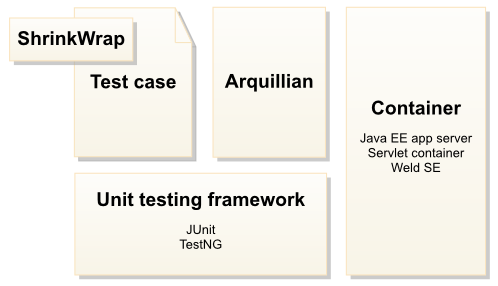
\includegraphics[width=60mm]{img/architecture-overview.png}
	\caption{The Arquillian test infrastructure}
	\label{fig:arquillian_test_infrastructure}
\end{figure}

	\section{Arquillian containers}
		\subsection{Remote container}
		\subsection{Managed container}
		\subsection{Embedded container}
		
	\section{Arquillian running modes}
		\subsection{Client mode}
		\subsection{In-container mode}

	\section{Anatomy of an Arquillian test}
		\subsection{Arquillian descriptor}
		\subsection{Arquillian test}
		\subsection{Deployment}
	\section{Test lifecycle}
	\section{Test enrichment}
	\section{Extensibility of Arquillian}
		\subsection{Arquillian container API}
		\subsection{Arquillian SPI}

\chapter{Design of Arquillian container}
	\chapter{Merging event driven extension into container context}
	
\chapter{Implementation of Arquillian Android container}

\chapter{Usage of Android container in web testing context}

	\section{Selenium WebDriver}
	
	\section{Arquillian Graphene}
	
	\section{Arquillian Drone}
	
	\section{Web testing with Android container}

\chapter{Native testing of Android application}

%	\section{Arquillian philosophy}
%When some code is being developed in the iteration of the XP development process, we have to assert that code is eventually working in %the final product environment. The obvious approach to be sure that what we coded behaves properly is to deploy whole applicati

\bibliographystyle{plain}  % bibliografický styl 
\bibliography{bib-db}      % soubor s citovanými
                           % položkami bibliografie 

\printindex

%%%%%%%%%%%%%%%%%%%%%%%%%%%%%%%
%
%       A P P E N D I X  
%
%%%%%%%%%%%%%%%%%%%%%%%%%%%%%%%

\appendix
\end{document}
